%-----------------------------------------------------------------------------%
%- Appendix :: Trig Identity Quickstart --------------------------------------%
%-----------------------------------------------------------------------------%
\chapter{Trig Identities}
\label{chap:TrigIdentities}
Inverse, quotient, angle sum, and the first primitive identity are the trig
identities are required to memorize. Everything else can be derived.\footnote{However, if you can memorize all of these identities, it may
save crucial seconds in test and exam situations.}

\section{Reciprocal Identities}
\label{sec:TrigReciprocalIdentities}
It should be worth noting the temptation to call these identities the ``inverse
identities'', however, this is technically not true. They are not a part of
MATH130 in any of the semesters I have done MATH130, however they will be
included for completeness at the end of this chapter in section
\ref{sec:TrigInverseIdentities}.
\begin{align}
  \rsin \theta = \frac{1}{\sin \theta} = \csc \theta\\
  \rcos \theta = \frac{1}{\cos \theta} = \sec \theta\\
  \rtan \theta = \frac{1}{\tan \theta} = \cot \theta
\end{align}

\section{Quotient Identities}
\label{sec:TrigQuotientIdentities}
\begin{align}
  \tan \theta = \frac{\sin \theta}{\cos \theta} \\
  \cot \theta = \frac{\cos \theta}{\sin \theta}
\end{align}

\section{Primitive Identities}
\label{sec:TrigPrimitiveIdentities}
Only the first primitive identity needs to eb memorized, remaining primitives
can be derived from the first.
\begin{align}
  \sin^2 \theta + \cos^2 \theta & = 1 \label{eq:TrigPrimitive}
\end{align}
\begin{align}
  \intertext{Divide \eqref{eq:TrigPrimitive} by $\sin^2$.}
  \sin^2 \theta + \cos^2 \theta & = 1 \nonumber \\
  \frac{\sin^2 \theta}{\sin^2 \theta} + \frac{\cos^2 \theta}{\sin^2 \theta}
    & = \frac{1}{\sin^2 \theta} \\
  1 + \cot^2 \theta
    & = \csc^2 \theta \label{eq:Trig2}
  \intertext{Divide \eqref{eq:TrigPrimitive} by $\cos^2$}
  \sin^2 \theta + \cos^2 \theta
    & = 1 \nonumber \\
  \frac{\sin^2 \theta}{\cos^2 \theta} + \frac{\cos^2 \theta}{\cos^2 \theta}
    & = \frac{1}{\cos^2 \theta} \\
  \tan^2 \theta + 1
    & = \sec^2 \theta \label{eq:Trig3}
\end{align}

\section{Angle Sum Identities}
\label{sec:TrigAngleSumIdentities}
Angle sum identities need to be memorized.
\begin{align}
  \sin(A \pm B)
    & = \sin{A}\cos{B} \pm \cos{A}\sin{B} \\
  \cos(A \pm B)
    & = \cos{A}\cos{B} \mp \sin{A}\sin{B} \\
  \tan(A \pm B)
    & = \frac{\tan{A}\pm\tan{B}}{1 \mp \tan{A}\tan{B}}
\end{align}
Angle sum identities form the basis for the double angle identities. There
should be no need to memorize the double angle identities as they can be derived
from the angle sum identities as $A = B = 2A$.

\section{Double Angle Identity: sin(2A)}
\label{sec:TrigDoubleAngleSin}
\begin{align}
  \sin(A + A)
    & = \sin(A)\cos(A) + \sin(A)\cos(A) \\
    & = 2\sin(A)\cos(A)
\end{align}

\newpage
\section{Double Angle Identity: cos(2A)}
\label{sec:TrigDoubleAngleCos}
\begin{align}
  \intertext{$\cos(2A)$ has 3 solutions we need to concern ourselves with in
  MATH130. The 2\tsup{nd} and 3\tsup{rd} solutions
  combine rearrangements of the primitive identity \eqref{eq:TrigPrimitive}.}
  \cos(A + A)
    & = \cos(A)\cos(A) - \sin(A)\sin(A) \\
    & = \cos^2(A) - \sin^2(A) \label{eq:TrigDAFirst}
    \intertext{Rearrange \eqref{eq:TrigPrimitive} to make $\sin^2(A)$ the
    subject}
    \sin^2(A) + \cos^2(A) & = 1 \nonumber \\
    \sin^2(A) & = 1 - \cos^2(A) \\
    \text{sub into \eqref{eq:TrigDAFirst}} \nonumber \\
    & = \cos^2(A) - \sin^2(A) \nonumber \\
    & = \cos^2(A) -(1 - \cos^2(A)) \\
    & = 2\cos^2(A) - 1
    \intertext{Rearrange \eqref{eq:TrigPrimitive} to make $\cos^2(A)$ the
    subject}
    \sin^2(A) + \cos^2(A) & = 1 \nonumber \\
    \cos^2(A) & = 1 - \sin^2(A) \\
    \text{sub into \eqref{eq:TrigDAFirst}} \nonumber \\
    & = \cos^2(A) - \sin^2(A) \nonumber \\
    & = (1 - \sin^2(A)) - \sin^2(A) \\
    & = 1 - 2\sin^2(A)
\end{align}

\newpage
\section{Double Angle Identity: tan(2A)}
\label{sec:TrigDoubleAngleTan}
\begin{align}
  \tan(A + A)
    & = \frac{\tan{A} + \tan{A}}{1 - \tan{A}\tan{A}} \\
    & = \frac{2\tan{A}}{1 - \tan^2{A}}
\end{align}

\section{Trigonometric Calculus Identities}
\label{sec:TrigCalculus}
Think of differentiation of trig functions as a loop with 4 steps, and each time
you differentiate, you have a different value which is fed into the next step of
differentiation. When you reach the last point, you are back where you
started.
\begin{align}
  \deriv{\sin{x}}{x}  & = \cos{x} \\
  \deriv{\cos{x}}{x}  & = -\sin{x} \\
  \deriv{(-\sin{x})}{x} & = -\cos{x} \\
  \deriv{(-\cos{x})}{x} & = \sin{x}
\end{align}
There are 4 quadrants to the unit circle, and differentiation is the process
where by we find the gradient of a function at a point $\theta$. Keep referring
back to figure \ref{fig:TrigCalcSinxCosx} for this next part:  
 \begin{figure}[!htb]
  \begin{center}
    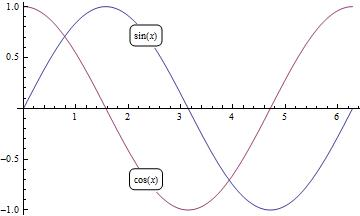
\includegraphics{img/sinxcosx}
    \caption{$\sin(x)$ and $\cos(x)$}
    \label{fig:TrigCalcSinxCosx}
  \end{center}
\end{figure}
\begin{enumerate}
  \item Consider the gradient of $\sin(0)$. $\sin(x)$ is at $(0,0)$ and it has a
  gradient that is at it's steepest: 1. Note how $\cos(0)=1$.
  \item Consider the gradient of $\sin(\frac{\pi}{2})$. $sin(x)$ is at a maximum
  at point $(\frac{\pi}{2},1)$, and the gradient is $0$. Note how
  $\cos(x)$ is plotted and when evaluated $\cos(\frac{\pi}{2})=0$.
  \item Consider the gradient of $\sin(\pi)$. $sin(x)$ is zero, and is at it's
  steepest ``downward slope''. Note how $\cos(x)$ is plotted and evaluated
  $\cos(\pi)=-1$.
  \item Consider the gradient of $\sin(\frac{3\pi}{2})$. $\sin(x)$ is at a
  minimum at point $(\frac{3\pi}{2},-1)$, and $\cos(x)$ is plotted and
  evaluated as $\cos(\frac{3\pi}{2})=0$.
\end{enumerate}
The next step would be to analyse the gradient of $\cos(x)$. One would find that
at any arbitrary point, the gradient of $\cos(x)$ will equal the value of
$\sin(x) \cdot -1$.

\section{Inverse Identities}
\label{sec:TrigInverseIdentities}
An inverse trig function can be though of as an ``undoing function'' for a trig
function.\footnote{This is much like how a logarithm is the undoing function for
an exponent.} All of the inverse trig functions are called
``arc<function>''. The inverse functions hold true iff $-\frac{\pi}{2} \leq
\theta \leq \frac{\pi}{2}$.
\begin{align}
  \sin(\arcsin \theta) &= \theta&\Longrightarrow&&\arcsin(\sin \theta)=\theta \\
  \cos(\arccos \theta) &= \theta&\Longrightarrow&&\arccos(\cos \theta)=\theta \\
  \tan(\arctan \theta) &= \theta&\Longrightarrow&&\arctan(\tan \theta)=\theta \\
  \sec(\arcsec \theta) &= \theta&\Longrightarrow&&\arcsec(\sec \theta)=\theta \\
  \csc(\arccsc \theta) &= \theta&\Longrightarrow&&\arccsc(\csc \theta)=\theta \\
  \cot(\arccot \theta) &= \theta&\Longrightarrow&&\arccot(\cot \theta)=\theta
\end{align}
